\chapter{Analiza tematu}

\paragraph{}
Aby rozpocząć działania nad projektem, w pierwszej kolejności należało przeanalizować problem. Ponadto, znaleziono podobne rozwiązania, które mogą być wzorem lub pomocą przy dążeniu do innowacyjnego  projektu.

\section{Sformułowanie problemu}

\paragraph{}
Aplikacja do śledzenia lokalizatorów może zostać stworzona w różnych językach progamowania. Może być również dostępna na różnego rodzaju urządzeniach, od urządzeń mobilnych, po komputery stacjonarne. Ważna jest również kompatybilność programu z konkretnym lokalizatorem. Niezbędne jest zastanowienie się nad tymi kwestiami, aby móc przejść do kolejnych kroków tworzenia aplikacji.

\section{Osadzenie tematu w kontekście aktualnego stanu wiedzy}

\paragraph{}
Wśród lokalizatorów dostępnych na rynku można znaleźć wiele rozwiązań. W zależności od ceny, możemy otrzymać dodatkowe funkcjonalności, mniej lub bardziej znaczące, są to między innymi czujnik wstrząsu, monitorowanie prędkości czy podsłuch. Producenci zazwyczaj posiadają własne strony internetowe, do których klient otrzymuje bezpłatny dostęp po zakupie produktu. Pozwalają one zwykle powiązać lokalizator z kontem użytkownika i śledzić na bieżąco jego lokalizację.

\paragraph{}
W celu stworzenia aplikacji do monitorowania lokalizatorów dla jak największej liczby ludzi, korzystających z tego typu urządzeń, warto przeanalizować kilka kwestii. Niezbędną funkcją lokalizatora jest możliwość jego konfiguracji, aby wysyłał dane na konkretny adres IP oraz port. Umożliwi to dostęp aplikacji do lokalizacji urządzenia. Szukane więc będą lokalizatory, do których można włożyć kartę SIM. Z tego powodu odrzucono produkty o najniższej cenie na rynku, gdyż nie oferują one wymaganej do działania programu funkcji. Przykładem jest Samsung SmartTag2, który nie umożliwia wysyłania danych lokalizacyjnych na konkretny adres. Kolejnym znaczącym aspektem wyboru lokalizatora jest jego cena w kontekście klienta. Należy wykluczyć najdroższe opcje, aby nie ograniczyć ilości potencjalnych użytkowników aplikacji. Model GP800+, któtego cena sięga powyżej sześciuset złotych, może być nieosiągalny dla wielu osób. Przykładami, które odpowiadają wyżej opisanym wymaganiom, są Coban TK108 lub Mking MK07A.

\paragraph{}
Podczas przeprowadzania analizy tematu, należało również wybrać stos technologiczny, w którym aplikacja będzie tworzona. Możliwe jest stworzenie aplikacji mobilnej, dostępnej przede wszystkim na smartfony, co wiąże się z wykorzystaniem języków programowania takich jak Flutter, React Native, Kotlin czy Swift. Kolejną opcją jest stworzenie aplikacji przeglądarkowej. Ten typ programów najczęściej pisany jest przy uzyciu języków: Java, Python, JavaScript.

\section{Opis znanych rozwiązań}

\paragraph{}
MKING GPS to aplikacja stworzona przez firmę Mking, posiadającą w swojej ofercie wiele modeli lokalizatorów GPS. Umożłiwia zarządzanie urządzeniami i jest dostępna jest wyłącznie na smartfony. Widok mapy w MKING GPS znajduje się na rys. \ref{mkinggps}  Chcąc utworzyć bardziej uniwersalny program, musiałby on być dostępny również na komputerach stacjonarnych czy też laptopach. Kolejnym przykładem jest platforma iTrackLive, będąca rozbudowaną aplikacją przeglądrkową - rys. \ref{itrack}. Niemniej jednak, liczba ikon i przycisków może przytłaczać zwykłego użytkownika. Aby ułatwić klientom uzytkowanie aplikacji, będzie ona prostsza w obsłudze, z mniejszą ilością funkcji, lecz ze schludniejszym interfejsem.

\begin{figure}
	\centering
	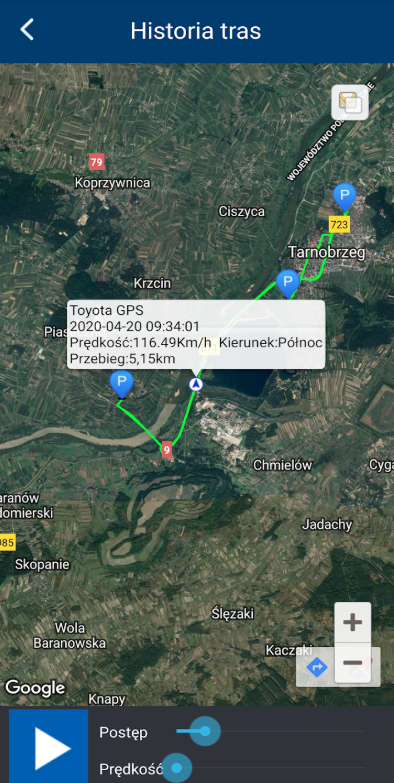
\includegraphics[width=0.6\textwidth]{./graf/mkinggps.png}
	\caption{Zrzut ekranu przedstawiający wygląd aplikacji MKING GPS.}
	\label{mkinggps}
\end{figure}

\begin{figure}
	\centering
	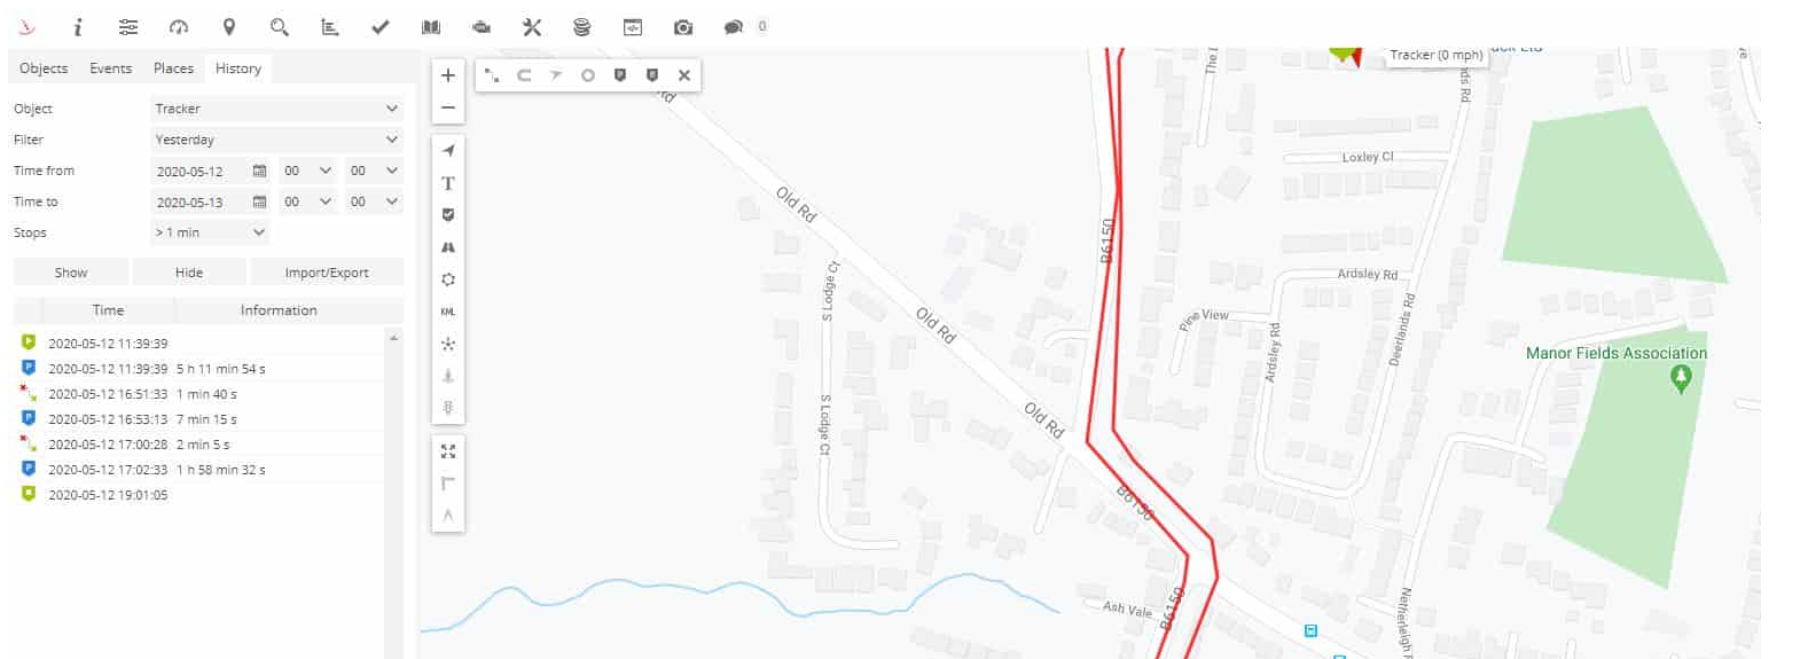
\includegraphics[width=1\textwidth]{./graf/itrack.png}
	\caption{Zrzut ekranu przedstawiający wygląd aplikacji iTrackLive.}
	\label{itrack}
\end{figure}